\documentclass[a4]{article}
\usepackage{LJMU-API}
\usepackage{parskip}
% Physics header taken from internet a long time ago, and manipulated to own ends along with some added bits below the original...

% ***********************************************************
% ******************* PHYSICS HEADER ************************
% ***********************************************************
% Version 2
\usepackage{multicol} % Allows for multiple columns

\let\vaccent=\v % rename builtin command \v{} to \vaccent{}
\renewcommand{\v}[1]{\ensuremath{\mathbf{#1}}} % for vectors

\newcommand{\gv}[1]{\ensuremath{\mbox{\boldmath$ #1 $}}} % for vectors of Greek letters
\newcommand{\uv}[1]{\ensuremath{\mathbf{\hat{#1}}}} % for unit vector

\newcommand{\abs}[1]{\left| #1 \right|} % for absolute value
\newcommand{\avg}[1]{\left< #1 \right>} % for average

\let\underdot=\d % rename builtin command \d{} to \underdot{}

\newcommand{\dif}[2]{\frac{d #1}{d #2}} % for derivatives
\newcommand{\ddif}[2]{\frac{d^2 #1}{d #2^2}} % for double derivatives

\newcommand{\pd}[2]{\frac{\partial #1}{\partial #2}} % for partial derivatives
\newcommand{\pdd}[2]{\frac{\partial^2 #1}{\partial #2^2}} % for double partial derivatives

\newcommand{\pdc}[3]{\left( \frac{\partial #1}{\partial #2} \right)_{#3}} % for thermodynamic partial derivatives

\newcommand{\ket}[1]{\left| #1 \right>} % for Dirac bras
\newcommand{\bra}[1]{\left< #1 \right|} % for Dirac kets
\newcommand{\braket}[2]{\left< #1 \vphantom{#2} \right| \left. #2 \vphantom{#1} \right>} % for Dirac brackets

\newcommand{\matrixel}[3]{\left< #1 \vphantom{#2#3} \right| #2 \left| #3 \vphantom{#1#2} \right>} % for Dirac matrix elements

\newcommand{\grad}[1]{\gv{\nabla} #1} % for gradient
\let\divsymb=\div % rename builtin command \div to \divsymb
\renewcommand{\div}[1]{\gv{\nabla} \cdot #1} % for divergence
\newcommand{\curl}[1]{\gv{\nabla} \times #1} % for curl

\let\baraccent=\= % rename builtin command \= to \baraccent
\renewcommand{\=}[1]{\stackrel{#1}{=}} % for putting numbers above =

%\newtheorem{prop}{Proposition}
%\newtheorem{thm}{Theorem}[section]
%\newtheorem{lem}[thm]{Lemma}
%\theoremstyle{definition}
%\newtheorem{dfn}{Definition}
%\theoremstyle{remark}
%\newtheorem*{rmk}{Remark}

% ***********************************************************
% ********************** END HEADER *************************
% ***********************************************************


\newcommand{\deriv}[2]{\frac{\mathrm{d}#1}{\mathrm{d}#2}}	
\newcommand{\pderiv}[2]{\frac{\partial #1}{\partial #2}}	
\newcommand{\psderiv}[3]{\frac{\partial ^2#1}{\partial #2\partial #3}}
\newcommand{\dd}{\ensuremath{\, \mathrm{d}}}
\newcommand{\e}{\ensuremath{\mathrm{e}}}
\newcommand{\ii}{\ensuremath{\mathrm{i}}}
\newcommand{\N}{\ensuremath{\mathbb{N}}}	
\newcommand{\Z}{\ensuremath{\mathbb{Z}}}	
\newcommand{\R}{\ensuremath{\mathbb{R}}}
\newcommand{\Q}{\ensuremath{\mathbb{Q}}}
\newcommand{\C}{\ensuremath{\mathbb{C}}}
%\DeclareMathAlphabet{\mathpzc}{OT1}{pzc}{m}{it}
\newcommand{\Rr}{\ensuremath{\mathcal{R}}}
\newcommand{\ve}[1]{\mathbf{#1}}
\newcommand{\st}{\ensuremath{^\mathrm{st}}}
\newcommand{\nd}{\ensuremath{^\mathrm{nd}}}
\newcommand{\rd}{\ensuremath{^\mathrm{rd}}}
\newcommand{\nth}{\ensuremath{^\mathrm{th}}}
	
\renewcommand{\vec}[1]{\overrightarrow{#1}}	
\renewcommand{\thefootnote}{\fnsymbol{footnote}}

\newcommand{\rect}{\ensuremath{\sqsubset\!\!\sqsupset}}
\newcommand{\comb}[2]{\ensuremath{^{#1}C_{#2}}}
\newcommand{\perm}[2]{\ensuremath{^{#1}P_{#2}}}

\DeclareMathOperator{\re}{Re}
\DeclareMathOperator{\im}{Im}
\DeclareMathOperator{\Log}{Log}
\DeclareMathOperator{\Arg}{Arg}
\DeclareMathOperator{\Wnd}{Wnd}
\DeclareMathOperator{\Res}{Res}
\DeclareMathOperator{\Ker}{Ker}
\DeclareMathOperator{\Orb}{Orb}
\DeclareMathOperator{\Stab}{Stab}
\DeclareMathOperator{\Fix}{Fix}

% Quantum Physics starts here:

\newcommand{\op}[1]{\ensuremath{\mathrm{\widehat{#1}}}}

\newcommand{\SE}{Schr\"{o}dinger equation }
\newcommand{\TISE}{time independent Schr\"{o}dinger equation }


%Quantum Physics ends here



%edit these to suit:
\myname{Group 38}
\mypid{}
\mycourse{CS4240 -- Deep Learning}
\mytma{ -- Blog Post}

%then do your stuff after the \begin{document} command

\title{EMR-CNN Paper Reproducibility Blog Post}
\author{
    Alexander Ivanov (a.p.ivanov@student.tudelft.nl, 6105025) \\
    Fedde van der Meer (f.vandermeer-1@student.tudelft.nl, 4749693) \\
    Pieter van Bentum (p.c.m.vanbentum@student.tudelft.nl 4694732) \\
    Wouter Boullart (w.l.c.p.boullart@student.tudelft.nl, 5042216)
}


\begin{document}
\maketitle

\section{Introduction}

This blog discusses an ensemble learning and slice fusion strategy that can be used for segmentation. First, the concept is explained using a application on three dimensional nuclei instances that was published by Liming Wu, Alain Chen, Paul Salama, Kenneth W. Dunn, and Edward J. Delp\footnote{L. Wu, A. Chen, P. Salama, K. W. Dunn and E. J. Delp, "An Ensemble Learning and Slice Fusion Strategy for Three-Dimensional Nuclei Instance Segmentation," 2022 IEEE/CVF Conference on Computer Vision and Pattern Recognition Workshops (CVPRW), New Orleans, LA, USA, 2022, pp. 1883-1893, doi: 10.1109/CVPRW56347.2022.00205.\label{original_paper}}. Then a replication of the strategy on fluorescence microscopy image segmentation is presented.

\section{EMR-CNN}

The proposed ensemble learning and slice fusion strategy for three-dimensional nuclei instance segmentation\footnotemark[1] uses a Ensemble Mask R-CNN (EMR-CNN) method. In this method, each 3D volume of dimensions \(X \times Y \times Z\) is denoted as $I$ and sliced into $Z$ 2D slices which are denoted as \(I_j \  \text{where} \  j \in \{1, ... , Z\}\). The method uses set of \(M\) 2D object detectors \(E\). \(E\) consists of individual detectors \(m_i\) where \(i \in \{1, ..., M\}\). The methods aims to fuse the 2D images (slices) \(I_j\) together to produce a 3D image \(I\).

For each slice the object detection results from detector \(m_i\) are stored as \(Det^{m_{i},z_{j}}\) which contains detected objects \(Det_{n}^{{m_i},z_{j}}\) where \(n \in \{1, ..., N_{det}^{m_{i},z_{j}}\}\) with \(N_{det}^{m_{i},z_{j}}\) being the total number of objects detected by detector \(m_{i}\) in slice \(I_j\). Each detection result \(Det_{n}^{{m_i},z_{j}}\) contains information on the segmentation mask, centroid, and confidence score of the detected object. These are respectively denoted as \(Seg_{n}^{{m_i},z_{j}},\ Ctr_{n}^{{m_i},z_{j}} \ \text{and} \Pr_{n}^{{m_i},z_{j}}\).

\(Det^{{m},z_{j}}\) are the 2D results for all detectors in \(E\) for slice \(I_j\), again containing information \(Seg^{{m},z_{j}}\), \(Ctr^{{m},z_{j}}\) and \(Pr^{m,z_j}\). The results are then fused to form \(Det^{z_{j}}\) with information  \(Seg^{z_{j}}\), \(Ctr^{z_{j}}\) and \(\Pr^{z_j}\) for image \(I_j\). Finally all \(Det^{z_j}\) are collected in \(Det^z\) which is then fused to form the final 3D result \(Det\) and \(Seg\), \(Ctr\) and \(Pr\). The ensemble fusion and slice fusion will be explained in the next section.

\subsection{Mask R-CNN detectors}

EMR-CNN trains a collection \(E\) of \(M\) similar Mask R-CNN\footnote{Kaiming He, Georgia Gkioxari, Piotr Dollár, \& Ross Girshick. (2018). Mask R-CNN.} detectors implemented by the \href{https://github.com/facebookresearch/detectron2}{Detectron2 platform}\footnote{\href{https://github.com/facebookresearch/detectron2}{https://github.com/facebookresearch/detectron2}\label{detectron2}}. The paper is not about the detectors themselves but about how to fuse multiple detector results into a single, better result.

\subsection{Fusion of detection results}

As mentioned before the proposed method fuses the 2D results from the detectors and uses that fusion to merge the 2D slices into a 3D volume. The proposed EMR-CNN uses the estimated confidence scores \(Pr^{m,z_{j}}\) to create a fused 2D segmentation for each slice. This fused segmentation \(Seg^{z_j}\) is then represented by a new probability map \(Pr^{z_j}\).

The first step in fusing the detection results is object matching. This is done using Ward's minimum variance implemented with Lance-Williams dissimilarity measures\footnote{Murtagh, F., \& Legendre, P. (2014). Ward’s Hierarchical Agglomerative Clustering Method: Which Algorithms Implement Ward’s Criterion? Journal of Classification, 31(3), 274-295. https://doi.org/10.1007/s00357-014-9161-z} to determine which masks can be merged. It quantifies the similarity between the existing cluster and a potentially merged cluster. Initially each detection is treated as a single cluster after which all clusters are extended or merged stepwise. In order to evaluate the performance of the clustering the mean intra and inter cluster distances, \(a(i)\) and \(b(i)\) respectively, are calculated.

\[a(i) = \frac{1}{n_c} \sum_{i,j \in C_c, i\neq j} d(i,j)  \quad\text{and}\quad b(i) = \frac{1}{k - 1} \sum_{q,q\neq c} \left( \frac{1}{n_q} \sum_{i\in C_c, j\in C_q} d(i,j)\right)   \]

Here \(a(i)\) quantifies the (Euclidean) distance between the centroid of mask \(i\) and that of the the other samples in its cluster \(C_c\). \(b(i)\) calculates the distance between the centroid of mask \(i\) and that of other clusters \(C_q\). Note that \(n_c\) denotes the number of elements in \(C_c\). As there are many possibilities for the number of clusters the Silhouette Coefficient \((SC_{z_j}\)) is calculated in order to get to an ideal number of clusters \(N^{\text{cluster}}_{z_j}\) for each slice \(z_j\). 
% In this application \(k_{\text{min}}\) needs to be at least 2.
To improve the robustness of this method all detections in cluster \(C_r\) will be removed if \(C_r\) contains less than \(M/2\) detections.

\[N^{\text{cluster}}_{z_j} = \underset{k}{\arg\max} SC_{z_j}(k), \ k\in \{k_{\text{min}},..., k_{\text{max}}\} \quad \text{where} \quad SC_{z_j}(k) = \frac{1}{k} \sum_{i \in Ctr^{m, z_j}} \frac{b(i) - a(i)}{\text{max}(a(i), b(i))} \]  \\ 


The final step in the 2D fusion is to fuse the masks from the \(M\) detectors together. This is done using a proposed weighted 2D mask fusion where \(C_w\) denotes the \(w\)-th cluster. 

\[Seg_w^{z_j} =\frac{\sum_{i \in C_w} Pr_i^{m, z_j} Seg_i^{m, z_j}}{\sum_{i \in C_w} Pr_i^{m, z_j}}>0.5 \quad \text{and} \quad Pr_w^{z_j}  =\frac{1}{\left|C_w\right|} \sum_{i \in C_w} Pr_i^{m, z_j}\] \\

\hrulefill \\

Now that the fused slice results \(Det^{z_j}\) have been established the slices can be fused into a 3D detection \(Det\). This is done using two approaches based on \(Ctr^{z_j}\). The first approach, blob-slice, merges the slices from top to bottom using a nearest neighbour chain created by a user-defined Euclidean distance between the \(Ctr^{z_j}\). The second method uses the clustering procedure as described before but applied to cluster the centroids \(Ctr^z\). \\

As all slices are fed to the detectors and 2D fusion independently of its position in the 3D volume, some slices may miss a detection that is present in the slices above and below. This would result in 2 smaller detections in 3D whereas there should only be 1 bigger detection. This problem is solved by fabricating the missing segmentation using the intersection of the two segmentation above and below.

\[Seg_r^{z_j} = Seg_p^{z_{j-1}}\cap Seg_q^{z_{j + 1}} \]\\


In summary, the masks are detected as follows. We have a lot of 3D images of cells. Each 3D image of the cells is sliced into a bunch of 2D slices. These 2D slices go into multiple detectors (we use 8). All these detectors use Mask R-CNN to try and label each cell in a slice. Next, the results of all the detectors (the ensemble) is combined (fused) into a single mask. Now we have a mask for every 2D slice. These 2D masks are then fused back into a 3D mask.

\section{Replication setup}

The code provided alongside the paper only runs under Linux and requires a powerful GPU (the authors worked with an NVIDIA Titan Xp 12GB). Therefore, in accordance with our course recommendations, we configured a Linux virtual machine with one NVIDIA Tesla T4 GPU in Google Cloud.

To ensure our project environment was portable and easy to reproduce, we used Docker containers with the NVIDIA NGC image\footnote{\url{https://catalog.ngc.nvidia.com/orgs/nvidia/containers/pytorch}} as a starting point. Furthermore, Detectron needs to be built from source\footnote{\url{https://detectron2.readthedocs.io/en/latest/tutorials/install.html}} to target newer PyTorch and CUDA versions, so choosing container images allowed us to reuse and distribute a code-ready environment that would have otherwise been very fragile.

In our GitHub repository\footnote{\url{https://github.com/sashoism/emrcnn-polarity}} we provide Docker Compose configurations that can be used to launch the train-test pipeline for a given dataset with a single command. One of the configurations tests with the pretrained weights in the archive provided in the original paper.

\subsection{Reproduction results}

Our setup is able to reproduce the model outputs of the authors on their example dataset.

\begin{figure}[h!]
    \centering
    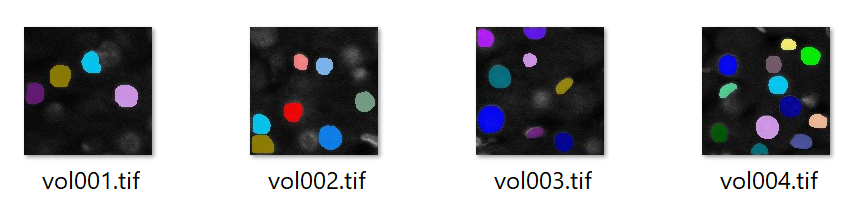
\includegraphics[width=0.85\textwidth]{figures/emrcnn-immu.png}
    \caption{Segmentation masks overlaid on the synthetic \texttt{immu} dataset}
    \label{fig:emrcnn-immu}
\end{figure}

\section{Application to yeast budding segmentation}
EMR-CNN was selected to be a good candidate in the problem of detecting the budding of yeast cells. Budding of yeast cells is indicated by a protein which is imaged by fluorescence microscopy. This protein can then be imaged as a timelapse of 3D grey scale images. An example of a 2D slice of one of the 3D images can be seen below.
\begin{figure}[h!]
    \centering
    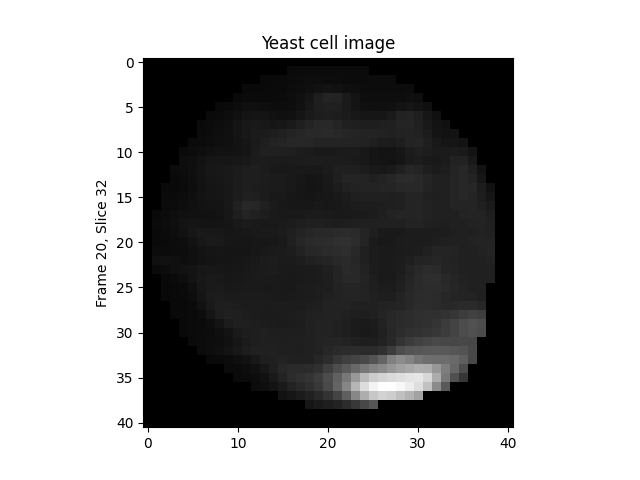
\includegraphics[width=0.6\textwidth]{figures/data.png}
    \caption{Original cell polarity data}
    \label{fig:enter-label}
\end{figure}

For training purposes, these images are manually segmented into foreground and background, resulting in a mask. The mask overlaid on top of the image can be seen below.

\begin{figure}[h!]
    \centering
    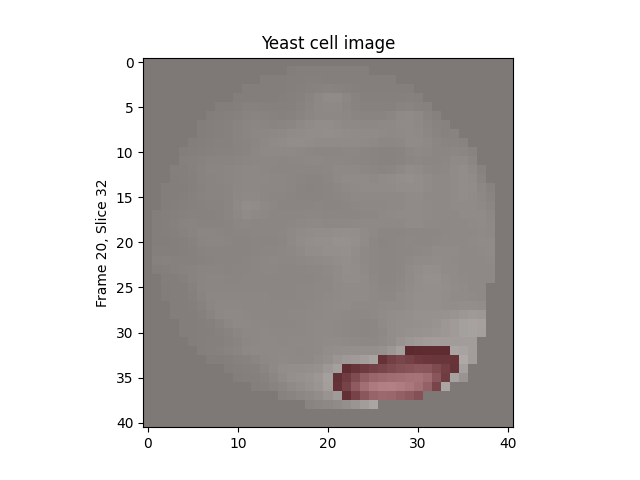
\includegraphics[width=0.6\textwidth]{figures/mask.png}
    \caption{Segmentation mask}
    \label{fig:enter-label}
\end{figure}

The goal is to train the EMR-CNN model to segment new data automatically. To do this, first the data was pre-processed. After this the model was split into a training and test set. Next, the model was trained on the training set. Finally, to assess the accuracy of the newly trained model it was applied to the test set.\\
The pre-processing of the data consisted of multiple steps.
The data contained 4D images, where every image represented a 3D volume over multiples time instances. First of all, the 4D images were split up into 3D volumes, as this is the dimensionality the model expects. Next some representative samples of the data were curated. This is done because it would take too long to train on all of the data. The selection was done by taking a single volume from each 4D image, which had a nonzero mask.\\
The data was also reshaped, using interpolation. This was done for two reasons. First, because all images had different dimensions and the model expected all images to have the same dimensions. Second, because the data has relatively high resolution we could save on training time by downsampling the images. This is of course at the cost of resolution and because of this the model might not recognise some small scale features.


\subsection{Discussion}
Unfortunately the model was not able to accurately detect and segment yeast budding. This is probably due to some fundamental differences between the problem of cell detection, which is the application used in the paper, and the problem of yeast budding detection. To explain this, let us look at the fundamental goal of EMR-CNN.\\
First of all, convolutional neural networks (CNN) can find features which predict whether there should be a mask or not. Next, region-proposal CNN (R-CNN) uses CNNs to propose multiple regions in an image in which an object might be. Already this is not the goal of the yeast budding problem as we are looking to segment a single object in a single region and therefore do not need to detect regions. Next, mask R-CNN segments each region into foreground and background, but since we have only a single region this might give issues. Finally ensemble mask R-CNN (EMR-CNN) uses an ensemble of multiple mask R-CNN detectors to come to a better result by using a voting mechanism.\\
From this we can conclude that the task of segmenting yeast budding images should be possible using just a CNN. Using EMR-CNN is more useful if the goal was to detect multiple budding yeast cells at the same time. From the paper the most useful part would be the 2D to 3D fusion, but it is probably better to just have a CNN that can segment 3D images.\\
For this reason we implemented a 3D CNN.

\section{3D CNN}

A 3D CNN model using the Keras library with a TensorFlow backend is constructed. The model architecture can be summarized as follows:
\begin{itemize}
    \item Input shape: (32, 32, 32, 1) - 3D data with dimensions 32x32x32 and a single channel (grayscale).
\item Three convolutional blocks, each followed by max-pooling:
\begin{itemize}
    \item First block: 32 filters of size 3x3x3, ReLU activation, same padding.
    \item Second block: 64 filters of size 3x3x3, ReLU activation, same padding.
    \item Third block: 128 filters of size 3x3x3, ReLU activation, same padding.
\end{itemize} 
\item Each max-pooling layer reduces the spatial dimensions by a factor of 2.
\item Flatten layer to convert the output of the convolutional blocks into a 1D array.
\item Two fully connected layers with ReLU activation: 256 neurons, then 128 neurons.
\item Dense layer with sigmoid activation to produce an output array of size 32x32x32 (similar to input shape).
\end{itemize}
The model aims to learn to generate binary masks for 3D data, where each voxel (3D pixel) is classified as either foreground or background. The final layer produces an output between 0 and 1 for each voxel, indicating the probability of it being part of the foreground object.\\
Finally the probabilities are converted to binary masks by setting all vlaues larger than 0.5 equal to 1, and all other values equal to 0.
\subsection{Loss function}
Initially, binary cross-entropy loss was considered as this is a common choice for binary segmentation tasks. However, it can struggle with imbalanced datasets, where one class significantly outnumbers the other. Our data is heavily unbalanced as around 99.7\% is the background class and only 0.3\$ is the foreground. This imbalance causes the loss function to prioritize the majority class, leading to poor sensitivity to the minority class. To address these issues, class weighting was applied, giving more weight to the smaller class. This however still resulted in classifying everything as the majority class i.e. the background.\\

The next loss function considered was Dice loss which is commonly used for binary classification tasks with imbalanced datasets. Dice loss is defined below\\

Dice coefficient:
\[ Dice = \frac{2  |X \cap Y|}{|X| + |Y|} \]

Dice loss:
\[ Dice\_Loss = 1 - Dice \]

Where \(X\) represents the set of voxels predicted as foreground by the model. \(Y\) represents the set of voxels labeled as foreground in the ground truth. \(|\cdot|\) denotes the number of elements of the set.

Dice loss encourages the model to produce segmentation masks with high spatial overlap with the ground truth masks, regardless of class imbalance. By focusing on spatial agreement, rather than class probabilities, Dice loss can mitigate the effects of imbalanced datasets and improve model performance.

\subsection{Results}
The model was trained for 40 epochs after which the loss curve seemed to plateau around a loss of 0.22 for the validation set.

\begin{figure}[h!]
    \centering
    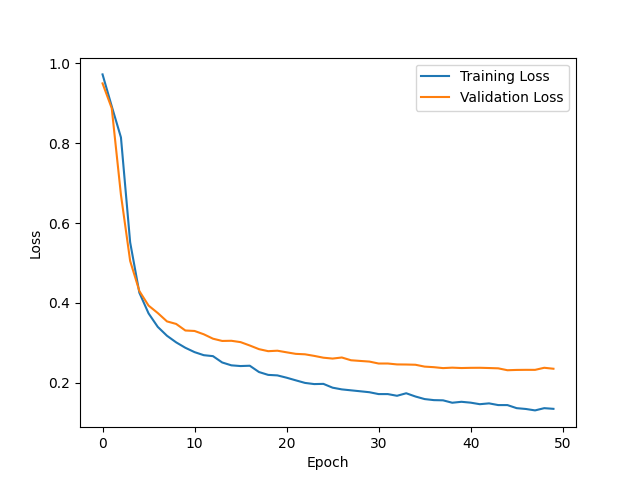
\includegraphics{figures/Loss_curve.png}
    \caption{Loss Curve}
    \label{fig:enter-label}
\end{figure}

The test set a similar loss to the validation set. Overlaying the cell data and actual mask with the predicted mask gives a good indication of how well the model performs. A typical example from the test set is shown below. The purple indicates the true mask, green indicates the predicted mask and dark grey indicates overlap between the two masks. The results on the test set can be in the table below.

\begin{table}[]
    \centering
    \begin{tabular}{|c|c|}
    \hline
         Loss&  0.2183\\
         \hline
         Accuracy& 0.9987\\
         \hline
         Mean IoU& 0.6268 \\
         \hline
    \end{tabular}
    \caption{Results on test set}
    \label{tab:my_label}
\end{table}

\begin{figure}[h!]
    \centering
    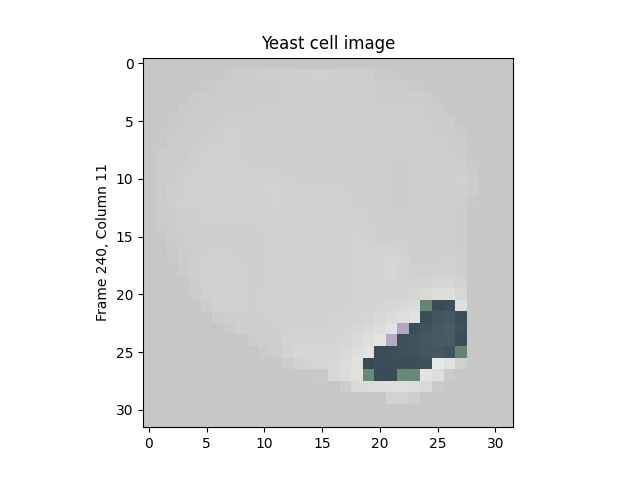
\includegraphics{figures/Cell_Pred.png}
    \caption{}
    \label{fig:enter-label}
\end{figure}

\section{Project Planning}
The project started with a kickoff meeting with the TA and external supervisor. The TA being the main supervisor for the project, and the external supervisor a sort of client for which we would do the yeast budding segmentation. After the kickoff the team met twice a week, of which once a week was a session in which the TA could be asked for advice. The tasks were divided as follows.
\begin{itemize}
    \item Investigating environment possibilities: Wouter, Pieter, Alex
    \item VM setup: Alex and Pieter
    \item Data pre-processing: Fedde and Alex
    \item Blog setup: Wouter
    \item Implementing researcher data: Fedde and Alex
    \item 3D CNN: Fedde
\end{itemize}
\end{document}